\documentclass[11pt,a4paper]{article}

\usepackage{microtype}
\usepackage{graphicx}
\usepackage{listings}
\usepackage{siunitx}
\usepackage{hyperref}
\usepackage{float}

\title{GPU Assignment}
\author{Jan van der Lugt}
\date{}

\begin{document}
\maketitle

\section{Introduction}
The report discusses my implementation of an image processing pipeline for the Parallel Programming Practical course. In this image processing pipeline, 4 steps can be identified:
\begin{enumerate}
\item Grayscale conversion
\item Histogram calculation
\item Contrast enhancement
\item Smoothing
\end{enumerate}
Section 2 will go through these steps and explain into detail how the specific kernel was converted to a CUDA kernel. Section 3 will report the overall speedup compared to sequential kernels and identify room for improvement.

\section{Image conversion pipeline}
All runtimes in this section are based on an image on in the image set. The image in the image set has `nice' dimensions, which makes the impact of `pitching' the memory hard to measure. Therefor, a big image found on Google Image search was used\footnote{\url{http://www.adnahome.org/xviews/town-1969-large.jpg}}. The dimensions of this image are 8773 x 5352 with 24-bit colors (total of 46.953.096 pixels).

Furthermore, only the kernel execution time is measured, memory copying is not taken into account. In a production environment, the image would not be copied from and to the GPU between every two kernels. In our case, this would mean changing the entire host program, which was not necessary to measure the kernel speedups.

The hardware used for these experiments is a Nvidia GTX 480, which has a theoretical arithmetic rate of 1345 GFLOPS (single precision) and a memory bus bandwidth of 177 GB/s. The CPU used is an Intel Xeon E5620 clocked at 2.40GHz.

\subsection{Grayscale conversion}
The grayscale conversion was the simplest of the four. A trivial conversion already yielded more than a factor 60 speedup compared to the CPU kernel. By adding a few optimizations, this could be increased to a factor 160 speedup.

The optimizations used were:
\paragraph{Memory coalescing}
Many threads are active at the same time, and the GPU hardware can group their memory request into bigger requests. This requires that the request are done in certain patterns. The Fermi hardware used for these experiments is quite good at grouping memory request compared to previous generations, which makes the speedup difficult to measure.

\paragraph{Memory fetch size increase}
It is possible to fetch 4 bytes at a time instead of 1 byte and process those bytes in one thread. This reduces the overhead of starting thread blocks, fetching memory, etc., since 4 times as much work is done for the same amount of overhead. It does make the code a little less nice, however. \\

\begin{tabular}{ | l | S | }
	\hline
	\textbf{Kernel type} & \textbf{Runtime (ms)} \\
	\hline                       
	CPU kernel & 293.1 \\
	\hline
	Naive GPU kernel & 4.7 \\
	\hline
	Memory coalescing & 4.6 \\
	\hline
	Memory coalescing and memory fetch size increase & 1.8 \\
	\hline
\end{tabular} \\

The last kernel has 39 operations in total for every 4 pixels that are processed. This includes operations for calculating where to load and store pixels from and to. Since the operation runs in 1.8 ms, this means we get an arithmetic rate of 254 GFLOPS, which is just under 19\% of the theoretical maximum.

A total of 16 bytes were transferred per 4 pixels, which brings the memory transfer rate to 104 GB/s, or 59\% of the theoretical maximum.

\subsection{Histogram calculation}
The second kernel was a lot more difficult to optimize. There are 256 different gray values in the image, which can be counted in a histogram. This histogram can then be used to determine the parameters for the next kernel, contrast enhancement.

This kernel uses three optimizations, namely the two used in the grayscale conversion, with an addition of a shared memory optimization.

\paragraph{Shared memory}
Since the histogram counts are a shared memory structure, it is very important to use the right memory types of the GPU. It is possible to use an array of 256 integers in the global memory and use atomic adds to increment them. This is the naive solution, but as it turns out, the performance is really bad. The cause is that all atomic adds have to be serialized, slowing down the computation tremendously.
It's already a lot better to use shared memory to store a temporary array of counters, which is added to the global array at the end of the threads' execution. \\

\begin{tabular}{ | l | S | }
	\hline
	\textbf{Kernel type} & \textbf{Runtime (ms)} \\
	\hline                       
	CPU kernel & 61.8 \\
	\hline
	A: Naive GPU kernel & 74.4 \\
	\hline
	B: A + Memory coalescing & 74.4 \\
	\hline
	C: B + Memory fetch size increase & 55.3 \\
	\hline
	D: C + Shared memory & 11.7 \\
	\hline
\end{tabular} \\

The final version of the kernel has 15 operations per set of 4 pixels and it runs in 11.7 ms. The arithmetic rate for this kernel is very low, only 15 GFLOPS (or just over 1\% utilization). The cause is the high number of atomic adds, which can not be parallelized. The speedup over the sequential version is thus only 5.3x.

The kernel could be sped up more by reading more pixels per thread, for example 16 instead of 4, since this would balance the atomic add better between shared and global memory: there are 4 times less shared memory arrays, which increases the pressure on them, but also relieves the global memory array by a factor 4.

Since only 8 bytes are transferred per 4 pixels (of which 4 atomic), the memory transfer rate is only 8 GB/s or 5\% of the maximum.

\subsection{Contrast enhancement}
The third kernel uses parameters acquired from the histogram calculated by the previous kernel. Using these parameters, the dynamic range of the image is increased, by `stretching' the pixel values so the full range of grayscale values is used.

Again, the two optimizations of the first kernel are used, together with a third one, namely the replacement of if-statements by minimum and maximum functions:

\paragraph{Branch reduction}
GPU's are known to handle branches very badly, which is inherent to their SIMD nature (multiple concurrent branches would not adhere to the \emph{Single} Instruction part of SIMD). In case of a branch, the threads in a thread block have to split into two, one part following one direction of the branch, the other following the second part. Since these executions have to be serialized, the run time is increased. Where possible, branches should be avoided and replaced by other constructs, in this case by minimum and maximum functions. \\

\begin{tabular}{ | l | S | }
	\hline
	\textbf{Kernel type} & \textbf{Runtime (ms)} \\
	\hline                       
	CPU kernel & 372.9 \\
	\hline
	A: Naive GPU kernel & 4.6 \\
	\hline
	B: A + Memory coalescing & 5.1 \\
	\hline
	C: B + Memory fetch size increase & 3.9 \\
	\hline
	D: C + Branch reduction & 3.2 \\
	\hline
\end{tabular} \\

The final version of the kernel performs 32 operations per 4 pixels (including overhead) and runs in 3.2 ms. This brings the arithmetic rate for this kernel to 114 GFLOPS, which is a utilization of about 8.5\%. The speedup over the sequential version is 117x.

8 bytes are transferred per 4 processed pixels, which brings the memory transfer rate to 29 GB/s, or 17\% of the maximum. 

\subsection{Smoothing}

The final filter was the most difficult to optimize. It smooths the image by averaging the value of every pixel based on its own value and the surrounding 24 pixels' values. A naive implementation would thus need to fetch 25 pixels from global memory to calculate one new pixel value. To get good performance, the following optimizations were implemented:

\paragraph{Shared memory}
To reduce the number of memory requests, shared memory has to be used, since threads in the same thread block need overlapping pixel values in order to calculate new pixel values. By reading a block of memory into shared memory before starting the stencil execution, the number of memory requests to global memory per thread block is reduced from 6.400 to 400, more than an order of magnitude.

The only difficulty is the borders: a border of width 2 around the pixels of the thread block has to be fetched as well, so these have to be distributed among the threads in the thread block, resulting in some blocks fetching 2 or 3 pixels instead of 1.

\paragraph{Kernel specialization}
Since the original kernel has to do quite a lot of bounds checking, a lot of branching would be involved. To avoid having a lot of branches in the code that is used for the bulk of the pixels, two kernels were written: one that does bound checking, but does not use shared memory and another that does not bounds checking, but does use shared memory. The former is used for the borders of the image, while the latter is used for the rest of the image. This yields a significant speedup. \\

\begin{tabular}{ | l | S | }
	\hline
	\textbf{Kernel type} & \textbf{Runtime (ms)} \\
	\hline                       
	CPU kernel & 3794.4 \\
	\hline
	A: Naive GPU kernel & 65.6 \\
	\hline
	B: A + Kernel specialization and shared memory & 14.0 \\
	\hline
\end{tabular} \\

The final version of the kernel performs 196 operations per pixel (including overhead) and runs in 14.0 ms. This brings the arithmetic rate for this kernel to 657 GFLOPS, which is a utilization of about 49\%. The speedup over the sequential version is 271x.

656 bytes are transferred per 256 pixels, which brings the global memory transfer rate to 9 GB/s (or 5\% of the maximum). It must be noted that most bytes are read from shared memory, so this low utilization is to be expected.

\section{Overall speedup}
All kernels together run in 30.7 ms, compared to 4521.5 ms for the sequential version, which gives us a speedup of 151x.

To make the comparison a little bit more fair, we should add some memory allocation and copying time for the GPU version. If we assume the images stay in the global memory in between kernels, but have to be copied to and from the GPU at respectively the start and the end of the program, we should add 54.6 ms (see the table below), which brings the overall speedup to 53x, which is still very decent. The memory transfer overhead would, however, be 64\% of the total run time. \\

\begin{tabular}{ | l | S | }
	\hline
	\textbf{Kernel (operation)} & \textbf{Runtime (ms)} \\
	\hline
	Grayscale (allocation) & 0.4 \\
	\hline
	Grayscale (copy to device) & 35.1 \\
	\hline
	Histogram (allocation) & 0.2 \\
	\hline
	Histogram (copy from device) & 0.0 \\
	\hline
	Contrast (allocation) & 0.2 \\
	\hline
	Smoothing (allocation) & 0.3 \\
	\hline
	Smoothing (copy from device) & 18.4 \\
	\hline
\end{tabular} \\

If we take a look at the composition of the total run time at the next page, we can see that the histogram calculation accounts for a disproportionally large portion of it. Combined with the utilization of 1\% for this kernel, this would be the most obvious place to further optimize the program. Reducing the collisions of atomic operations on shared memory can be reduced, which will lower the contention and speed up the kernel.

\begin{figure}[t]
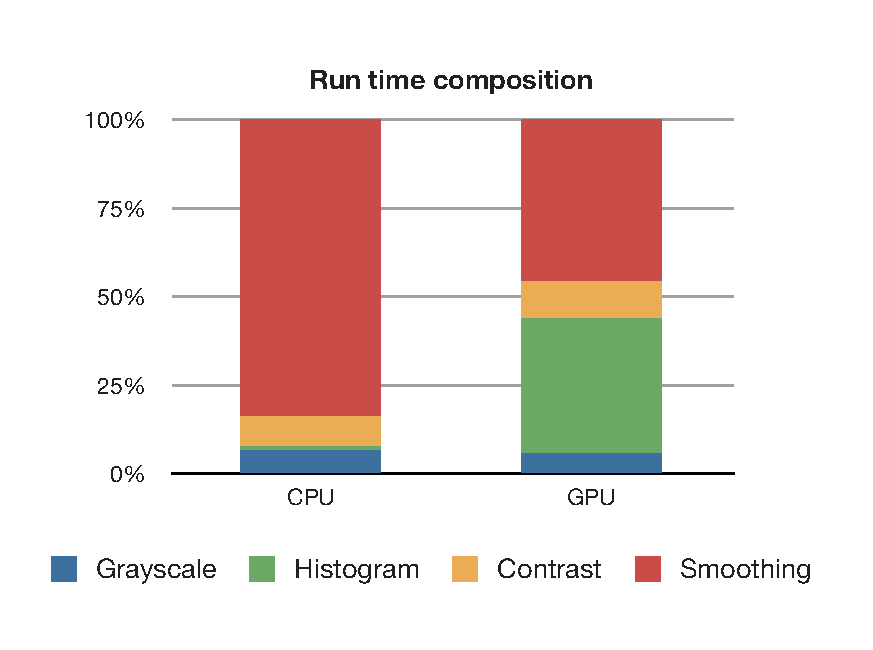
\includegraphics[scale=0.8]{figures/composition.pdf}
\end{figure}

\end{document}
